\section{Analysis Layer~1 ---  Mapping the Design Space Dimensions}
\label{sec:ch5-layer1}

This section charts the design space of future biophilic experiences imagined for indoor environments \textbf{(RQ1)}. It provides an overview of which experiential qualities were articulated, how they were expressed, and how widely different configurations of biophilic experience were explored across the sessions. We identified six design concepts (see \autoref{apx-design-concepts}), used as organising anchors to collate the dataset. We then developed seven analytic dimensions and associated codes using Krippendorff's~\cite{krippendorff2018content} content analysis. This section introduces these dimensions and their distributions, and visualises how coded qualities occur across the corpus using a multidimensional design-space map.

\subsection{The Design-Space Dimensions}
We first explain the seven dimensions. Detailed definitions and codes are in the codebook (\autoref{apx-sec-codebook}). \emph{Sensory Modality} captures the bodily channels through which experience is perceived (e.g. visual, auditory); \emph{Spatial Context} situates the experience within an architectural setting; \emph{Interaction Type} describes how occupants interact with the environment; \emph{Affective Aim} denotes the emotional goal in relation to the design (e.g. curiosity, vitality); \emph{Natural Reference} identifies the ecological phenomena drawn upon to frame or inspire the experience; \emph{Temporal Behaviour} characterises how experiential qualities occur over time. Finally, \emph{Level of Mediation} captures who/what shapes biophilic qualities (e.g. architectural form or technological systems). 

% The dimensions are a structured set of analytic axes that enable comparison and recombination across design concepts. Each dimension captures a distinct aspect of how biophilic interaction is specified, allowing experiential configurations to be described relationally (e.g. modality × interaction type × spatial context) rather than as isolated features. In this sense, the design space supports both analysis and generation by making these configurations comparable across otherwise dissimilar concepts.}

\paragraph{Sensory Modality}
Visual modalities were most prominent \emph{(n=82)}, followed by kinesthetic experience \emph{(n=71)}, including bodily effort, balance, gait, and movement. Auditory \emph{(n=53)} and tactile \emph{(n=47)} modalities appeared, often combined with movement or visual variation. Olfactory \emph{(n=5)} and taste \emph{(n=1)} were referenced very infrequently. 

\paragraph{Spatial Context}
Atriums \emph{(n=61)}, workstations \emph{(n=60)}, and staircases \emph{(n=45)} were most frequently referenced, reflecting an emphasis on spaces of movement, transition, and routine occupation. Outdoor-adjacent spaces \emph{(n=34)} (e.g. fa\c{c}ades) and corridors \emph{(n=33)} also featured prominently, highlighting interest in spatial edges and connective zones. Lounges \emph{(n=27)} appeared less frequently. 

\paragraph{Interaction Type}
Attending, sensory exposure without overt action, was the most prevalent mode \emph{(n=113)}, followed by traversing interactions \emph{(n=58)}, where variation is encountered through bodily movement across space. Handling captured direct physical engagement with materials or elements \emph{(n=45)}, such as curtains, textures, or stepping features. Reciprocal adjusting-to interactions \emph{(n=30)} and explicit coordination with others \emph{(n=14)} appeared occasionally, as secondary effects of shared occupation or navigation. 

\paragraph{Affective Aim}
Curiosity or gentle fascination \emph{(n=43)} was most frequently articulated, followed by natural vitality or aliveness \emph{(n=36)}, playfulness or light delight \emph{(n=36)} and empathy \emph{(n=35)}. Mental reset \emph{(n=32)}, comfort or safety \emph{(n=21)}, and authenticity or groundedness \emph{(n=23)} appeared at moderate levels, while calm \emph{(n=18)} and socialness \emph{(n=16)} were referenced more selectively. 

\paragraph{Natural Reference.}
Ground texture was the dominant reference \emph{(n=58)}, followed by vegetation \emph{(n=48)} and natural randomness or disorder \emph{(n=45)}. Water featured consistently across concepts \emph{(n=32)}, supporting both sensory and temporal variation. Atmospheric phenomena such as seasonality \emph{(n=25)}, airflow \emph{(n=19)}, and light and shadow \emph{(n=17)} appeared less often. References to landscapes or distant horizons \emph{(n=11)} and animal life \emph{(n=5)} were rare. 

\begin{figure*}[p]
  \centering
  \rotatebox{90}{%
    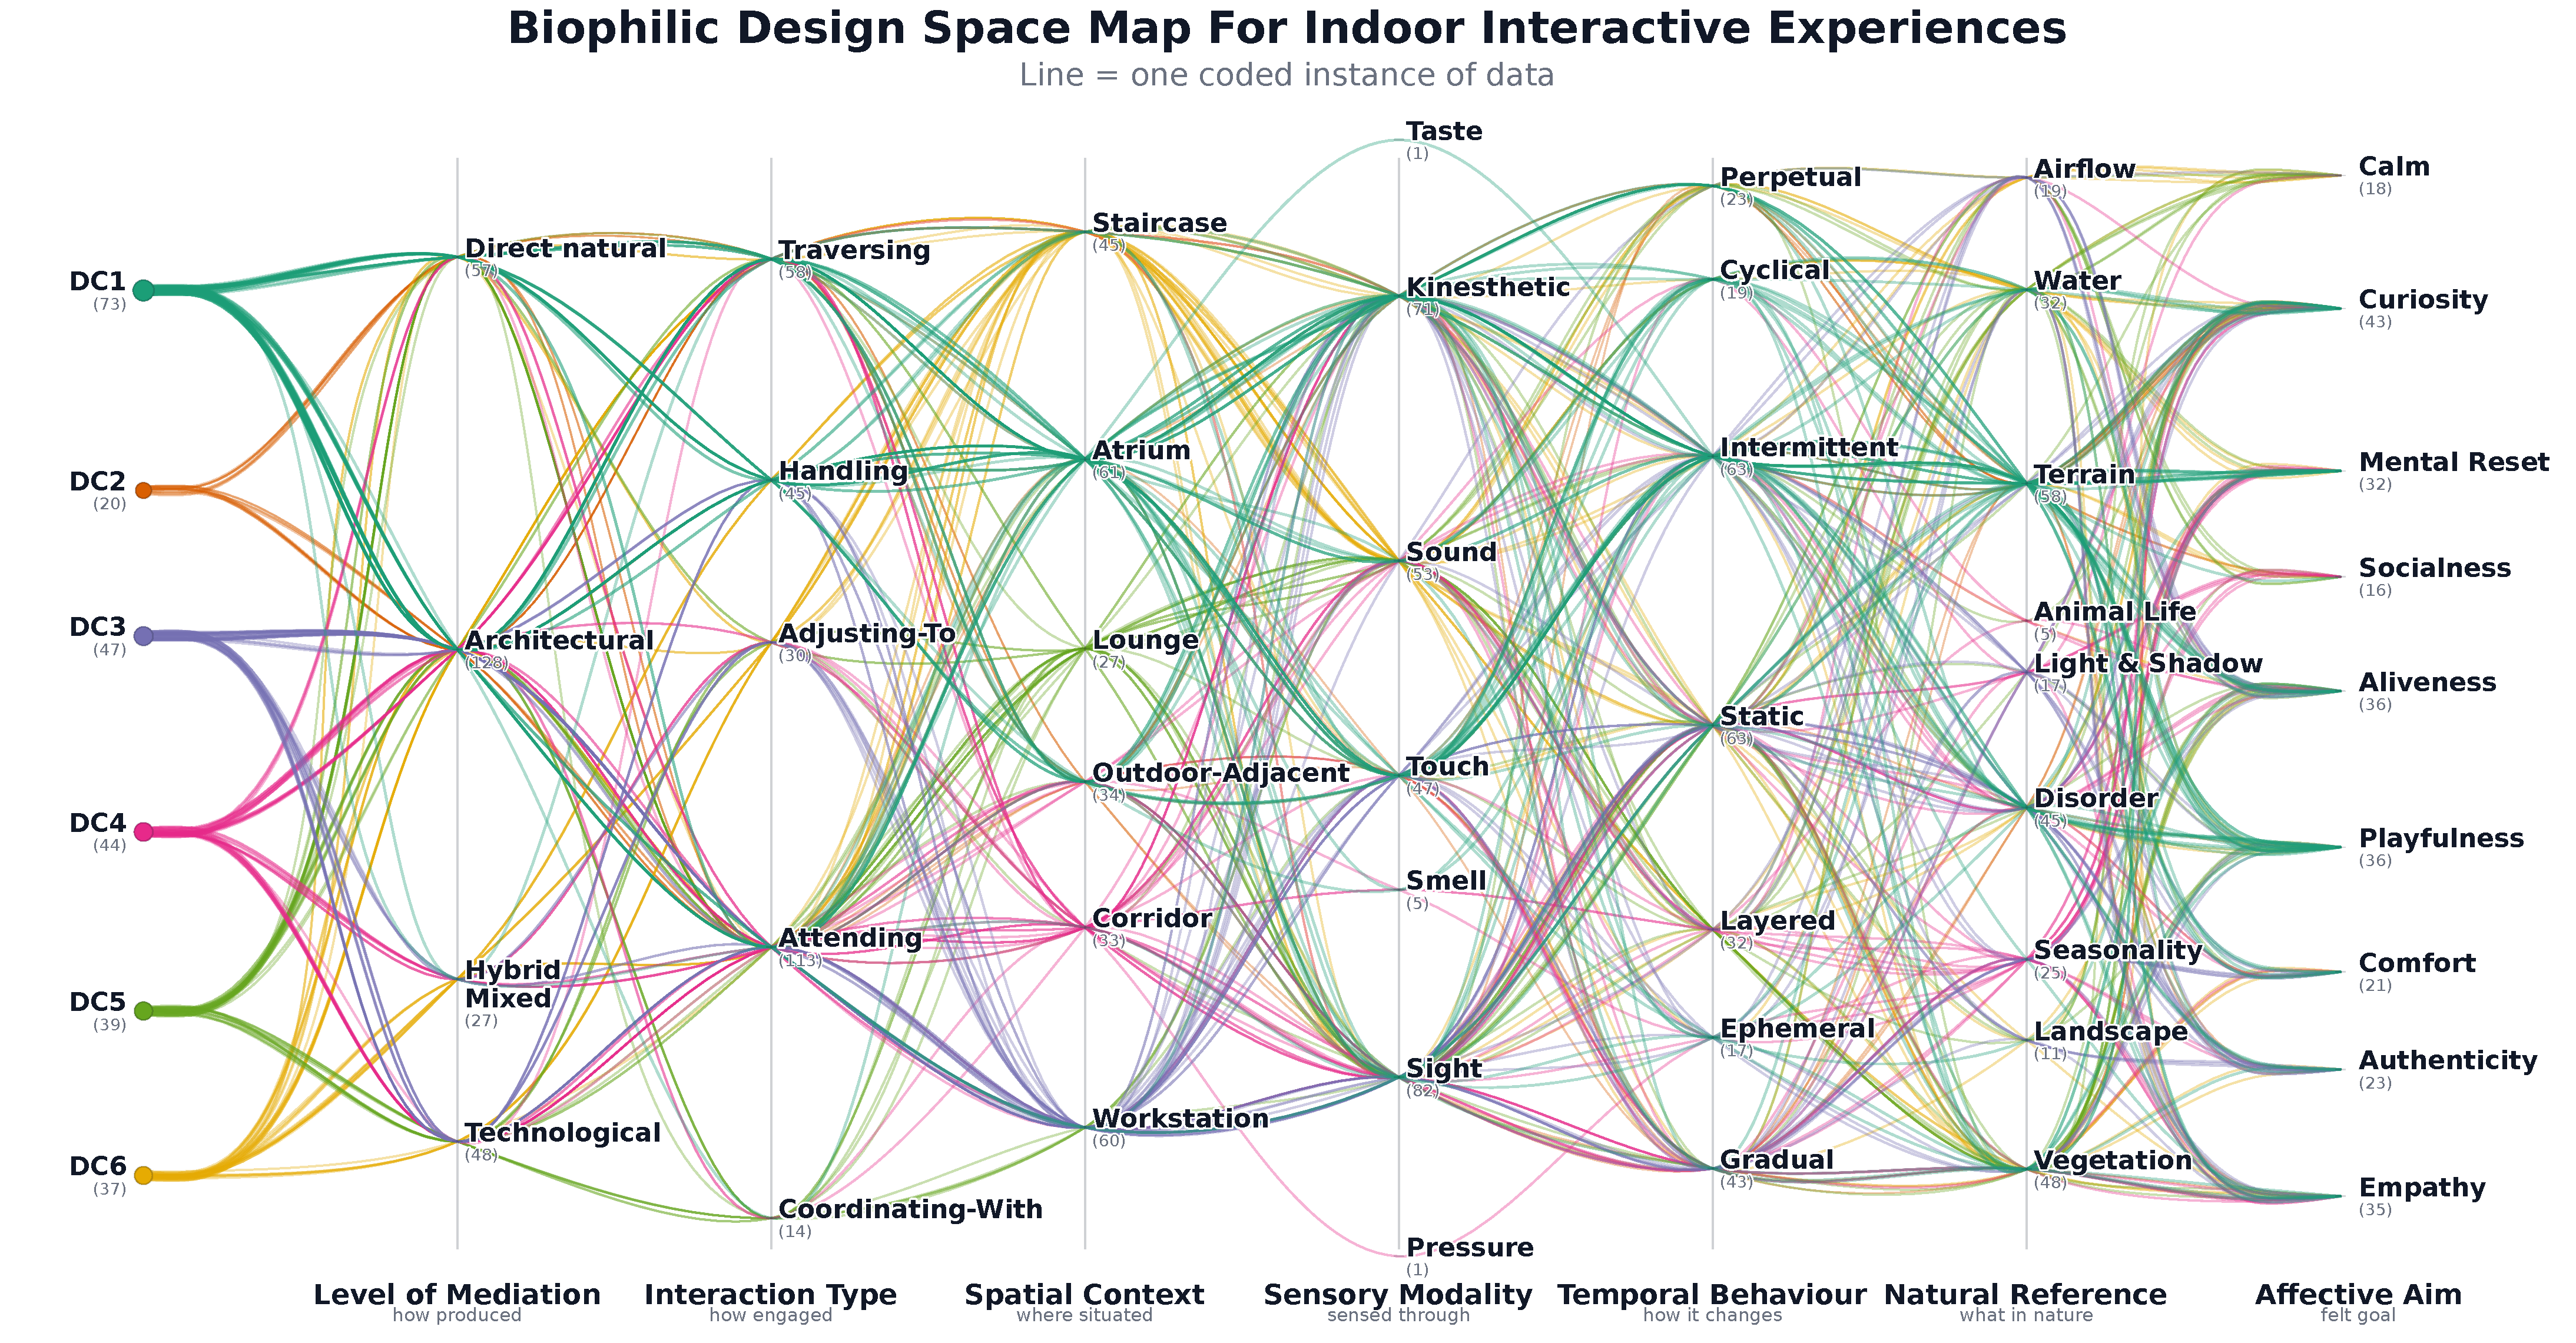
\includegraphics[width=0.89\textheight]{images/biophilic-map (6).pdf}
  }
  \caption{Biophilic design-space map showing how biophilic experiences were articulated across the expert design sessions. Each line represents a single coded statement and traces its assigned values across the seven analytic dimensions. Lines are coloured by their originating design concept to indicate provenance and conversational context, not analytic grouping. Line density and bundling indicate recurring combinations of experiential qualities, while dispersion reflects diversity in how biophilic experiences were imagined for indoor environments.}
  \Description{A biophilic design-space map visualising how biophilic experiences were articulated across the expert design sessions. Each line represents a coded statement traced across seven analytic dimensions. Line colour indicates the originating design concept, while line density and bundling show recurring experiential configurations and dispersion reflects diversity in imagined indoor biophilic experiences.}
  \label{fig:biophilic-map}
\end{figure*}

\paragraph{Temporal Behaviour}
Static \emph{(n=63)} and intermittent/sporadic variation \emph{(n=63)} were most common. Gradual change \emph{(n=43)} was also prominent, introducing irregularity and slow drift into otherwise static environments. Layered temporalities \emph{(n=32)} and perpetual behaviours \emph{(n=23)} appeared less frequently, while cyclical rhythms \emph{(n=19)} and ephemeral moments \emph{(n=17)} were rare. 

\paragraph{Level of Mediation}
Biophilic experiences were most commonly shaped through architectural mediation \emph{(n=128)}, where built form filters, frames, or structures natural qualities via materials, apertures, and spatial organisation. Direct encounters with unfiltered natural phenomena were also present \emph{(n=58)}. Technological mediation appeared selectively \emph{(n=48)}, in relation to sound or airflow. Hybrid mediation, combining architectural, technological, and natural layers, occurred least frequently \emph{(n=27)}. 

\subsection{The Multidimensional Design-Space Map}
Figure~\ref{fig:biophilic-map} visualises the coded dataset as a multidimensional design-space map, and \autoref{apx-design-concepts} shows the map for the three sessions. Each line represents one coded statement and traces its assigned values across the seven dimensions. Lines are coloured by originating design concept to indicate provenance, not grouping. Collectively, line density and bundling indicate how frequently particular configurations of qualities co-occur within and across concepts. Dense regions suggest recurring combinations of experiential qualities, while broader spread along an axis indicates greater variation within that dimension. The map functions as a descriptive cartography of the biophilic design space explored in the sessions, making visible which experiential qualities were repeatedly foregrounded, which were explored more selectively, and how individual concepts span multiple dimensions. 



\paragraph{Key Observations On Patterns of Convergence and Dispersion in Map}
\label{subsec:ch5-key-observations}

Several dimensions show strong convergence across concepts. \emph{Architectural mediation} is most employed, describing biophilic qualities shaped through spatial organisation, material articulation, or environmental filtering rather than through direct exposure or purely technological means. Interaction types oriented toward receptive or movement-based engagement, such as \emph{attending} and \emph{traversing}, also recur across concepts. Sensory modality similarly converges around visual and kinaesthetic channels, with many instances combining sight, movement, and bodily orientation.

In contrast, other dimensions display broader dispersion. \emph{Affective aim} spans range of experiential orientations, with instances distributed across curiosity, vitality, mental reset, comfort, and related registers rather than concentrated around a single affective outcome. \emph{Natural reference} likewise disperses across terrain, vegetation, water, atmospheric conditions, and irregularity, indicating that concepts draw on varied ecological sources rather than a shared biophilic motif. \emph{Temporal behaviour} exhibits a mixed pattern, with static and intermittent conditions appearing frequently alongside more selective use of gradual, layered, or ephemeral temporalities. 

Cross-dimensional patterns show interaction articulated within transitional spaces such as corridors, staircases, and atriums, where biophilic experience is embedded within movement across space rather than located at discrete points of engagement. Interaction is predominantly through \emph{architectural mediation} and described as exposure to or encounters with environmental qualities, with limited emphasis on reciprocal adjustment or direct control. \emph{Natural reference} frequently combines terrain, disorder, and atmospheric variation alongside vegetation, reflecting a focus on environmental processes rather than object-based representations alone. \emph{Temporal behaviour} is characterised by intermittent, gradual, and layered changes, structured through irregular or unfolding conditions rather than continuous or cyclical transformation.

\subsection{Conclusion}
Layer~1 surfaces which forms of sensing, interaction, temporality, ecological reference, and mediation were foregrounded, and where variation emerged. This layer is descriptive: it does not assess desirability or prioritise particular configurations. The patterns reframe interaction as arising through being-in and moving-through an environment. Interaction occurs across spatial trajectories rather than tied to interfaces. Environmental conditions are structured by the system, with occupants entering and negotiating them rather than triggering immediate responses. Biophilic references are through environmental processes (e.g. airflow, variability, disorder) rather than object-based representations. Temporal experience occurs gradually or intermittently, rather than through discrete events.